\documentclass[12pt]{article}

% Maths
\usepackage{amsmath}
\usepackage{amssymb}
\usepackage{bbm} % indicator function

% For (short)intertext
\usepackage{mathtools}

% Hyperlink
\usepackage{hyperref}
\hypersetup{
    colorlinks=true,
    linkcolor=blue,
    filecolor=magenta,      
    urlcolor=blue,
    pdfpagemode=FullScreen,
}

% Figures
\usepackage{graphics, float, subfig}
\usepackage[pdflatex]{graphicx}

% For custom environments
\usepackage{environ}

% Custom Environments
\NewEnviron{a_eq*}{\begin{center} \begin{align*} \BODY \end{align*} \end{center}}
\NewEnviron{a_eq}{\begin{center} \begin{align} \BODY \end{align} \end{center}}
\NewEnviron{c_eq*}{\begin{center} \begin{gather*} \BODY \end{gather*} \end{center}}
\NewEnviron{c_eq}{\begin{center} \begin{gather} \BODY \end{gather} \end{center}}
\NewEnviron{my_mp}{\begin{minipage}{\textwidth} \BODY \end{minipage}}

% Code
\usepackage{listings}
\usepackage{xcolor}
\definecolor{codegreen}{rgb}{0,0.6,0}
\definecolor{codegray}{rgb}{0.5,0.5,0.5}
\definecolor{codepurple}{rgb}{0.58,0,0.82}
\definecolor{backcolour}{rgb}{0.95,0.95,0.92}
\lstdefinestyle{mystyle}{
    backgroundcolor=\color{backcolour},   
    commentstyle=\color{codegreen},
    keywordstyle=\color{magenta},
    numberstyle=\tiny\color{codegray},
    stringstyle=\color{codepurple},
    basicstyle=\ttfamily\footnotesize,
    breakatwhitespace=false,         
    breaklines=true,                 
    captionpos=b,                    
    keepspaces=true,                 
    numbers=left,                    
    numbersep=5pt,                  
    showspaces=false,                
    showstringspaces=false,
    showtabs=false,                  
    tabsize=2
}
\lstset{style=mystyle}


% Itemize
\renewcommand{\labelitemi}{\textbullet}
\renewcommand{\labelitemii}{\textbullet}
\renewcommand{\labelitemiii}{\textbullet}

% Margins
\usepackage[margin=1in]{geometry}

%colors for questions
\usepackage{xcolor}

% Custom Commands
\renewcommand{\P}{\mathbb{P}}
\newcommand{\R}{\mathbb{R}}
\newcommand{\Z}{\mathbb{Z}}
\newcommand{\E}{\mathbb{E}}
\newcommand{\N}{\mathcal{N}}
\newcommand{\V}{\mathbb{V}}
\newcommand{\D}{\mathcal{D}}
\newcommand{\X}{\mathbf{X}}
\newcommand{\x}{\mathbf{x}}
\newcommand{\y}{\mathbf{y}}
\newcommand{\Y}{\mathbf{Y}}
\newcommand{\w}{\mathbf{w}}
\newcommand{\z}{\mathbf{z}}
\newcommand{\bd}{\boldsymbol{\delta}}
\newcommand{\0}{\boldsymbol{0}}
\newcommand{\1}{\boldsymbol{1}}
\renewcommand{\L}{\mathcal{L}}
\newcommand{\bq}{\bullet\quad}

% Title
\title{CSE 599B: Homework 3 Submission}
\author{Alexey Yermakov}
\date{May 31, 2024}

\begin{document}

\maketitle

\section{Random MPC with Shooting}

\begin{itemize}
    \item The reward during training with default hyperparameters for Random MPC with Shooting is plotted below:

    \begin{figure}[H]
        \centering
        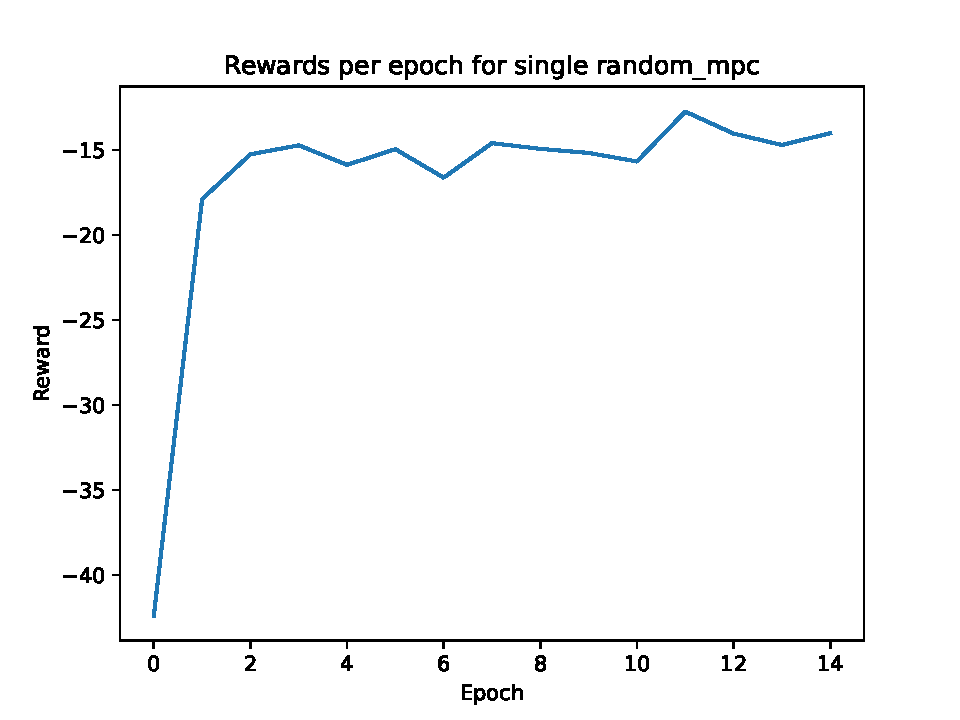
\includegraphics[width=.7\linewidth]{../figs/single_random_mpc.pdf}
        \caption{Reward per epoch with default hyperparameters for Random MPC with Shooting.}
        \label{fig:fig1}
    \end{figure}

    \item The success rate and average reward for Random MPC with Shooting with default hyperparameters is:
    \begin{verbatim}
Success rate:  0.41
Average reward (success only):  -13.303889559240533
Average reward (all):  -14.45317813467756
    \end{verbatim}
\end{itemize}

\newpage

\section{Model Predictive Path Integral (MPPI)}

\begin{itemize}
    \item The reward during training with default hyperparameters for MPPI is plotted below:

    \begin{figure}[H]
        \centering
        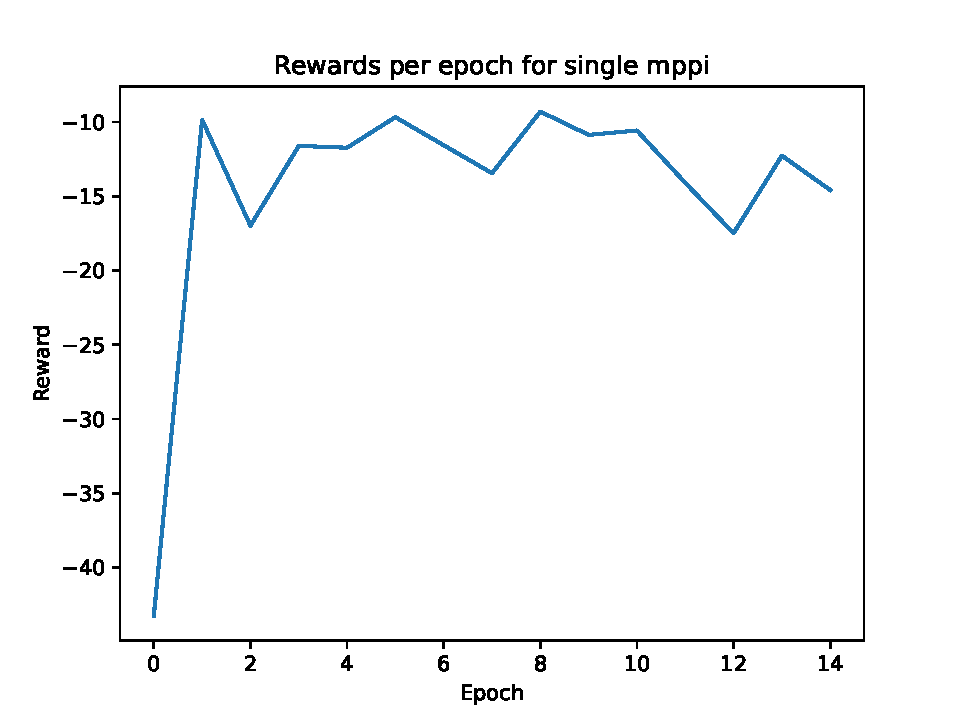
\includegraphics[width=.7\linewidth]{../figs/single_mppi.pdf}
        \caption{Reward per epoch with default hyperparameters for MPPI.}
        \label{fig:fig1}
    \end{figure}

    \item The success rate and average reward for MPPI with default hyperparameters is:
    \begin{verbatim}
Success rate:  0.37
Average reward (success only):  -9.265817016106594
Average reward (all):  -12.27599838847684
    \end{verbatim}
\end{itemize}

\newpage

\section{Esnemble MPPI}

\begin{itemize}
    \item The reward during training with default hyperparameters for ensemble MPPI is plotted below:

    \begin{figure}[H]
        \centering
        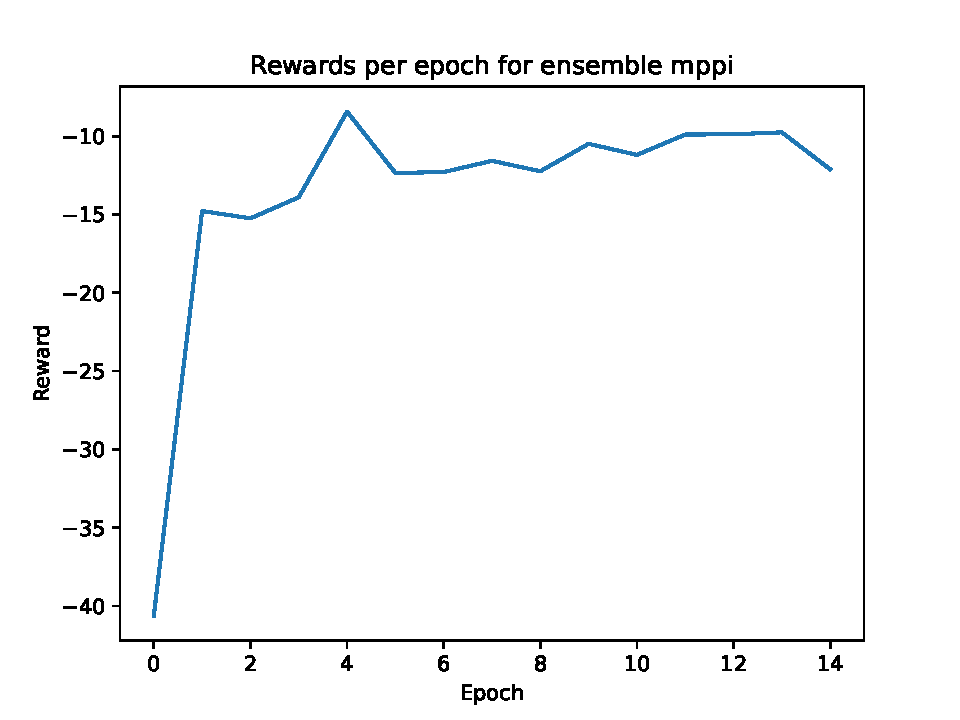
\includegraphics[width=.7\linewidth]{../figs/ensemble_mppi.pdf}
        \caption{Reward per epoch with default hyperparameters for ensemble MPPI.}
        \label{fig:fig1}
    \end{figure}

    \item The success rate and average reward for ensemble MPPI with default hyperparameters is:
    \begin{verbatim}
Success rate:  0.41
Average reward (success only):  -9.288529749275632
Average reward (all):  -11.397747670089936
    \end{verbatim}
\end{itemize}

\newpage

\section{Discussion}

\begin{itemize}
    \item[1.] Observing the performance of Random MPC with shooting, MPPI, and Ensemble MPPI leads to several key conclusions. First of all, the success rate for the reacher task is approximately the same for all three tasks from when I ran the code, at about 40\%. However, the average reward of the MPPI based methods are much higher than the random shooting. This makes sense since the random shooting is a random search and MPPI is much more of an informed. However, this informed search comes at the cost of runtime and code complexity. Random shooting ran in 1 minute and 3 seconds, single model MPPI ran in 6 minutes and 52 seconds, while ensemble MPPI ran in 29 minutes and 17 seconds. So, the improvement in reward for using MPPI came at the cost of runtime, which makes sense. However, the difference between single MPPI and ensemble MPPI was marginal in my results: an approximately the same average reward and a 4\% success rate improvement for the ensemble. This marginal improvement, however, came at the cost of running the code 5 times longer (the number of ensemble models used)!
    \item[2.] Diversity is important in an ensemble model because it helps promote searching diverse paths when doing path planning. If all the models were the same, the ensemble would do nothing to improve performance - the planning phase of the reinforcement learning loop would just take longer to run. Thus, in this homework I implemented varying batch sizes and learning rates used during model training for each model in the ensemble.
\end{itemize}

\end{document}